\documentclass[11pt]{article}
\usepackage{geometry} % see geometry.pdf on how to lay out the page. There's lots.
\usepackage{hyperref}
\usepackage{graphicx}
\usepackage{gensymb}
\usepackage[affil-it]{authblk}
\usepackage[toc,page]{appendix}
\usepackage{pifont}
\usepackage{amsmath}
\usepackage{amsthm}

\usepackage{float}

\newtheorem{theorem}{Theorem}
\newtheorem{corollary}{Corollary}
\newtheorem{conjecture}{Conjecture}
\newtheorem{proofsketch}{Proof Sketech}
\usepackage{draftwatermark}

\SetWatermarkText{DRAFT}
\SetWatermarkScale{6}
\SetWatermarkLightness{0.95}

% \geometry{letter} % or letter or a5paper or ... etc
% \geometry{landscape} % rotated page geometry

% See the ``Article customise'' template for come common customisations

\title{Untwisting the Tetrahelix (v0.4)}
\author{Robert L. Read \texttt{read.robert@gmail.com} \and
  Robert Gatliff \texttt{robert@toubat.org}
}


\date{\today}

%%% BEGIN DOCUMENT
\begin{document}

\maketitle

%% \tableofcontents

\begin{abstract}
  The Boerdijk--Coxeter helix (BC helix, or tetrahelix) is a face-to-face stack of regular tetrahedra.
  Considering the edges of these tetrahedra, the resulting structure is attractive and inherently rigid,
  and therefore interesting to architects, mechanical engineers,
  and robotocists.
  A formula that matches the visually apparent helices forming the outer rails of the tetrahelix is derived which
  is convenient for designers.
  This formula defines the vertices of tetrahelices of varying radius, pitch, and curvature, with the BC helix
  as a special case. 
  An addtional special case is of that of $0$ curvature or rail angle, which generates a \emph{tetrabeam}.
  A particular choice of paramaters defines a novel object, the  minimax member length-difference tetrabeam,
  the \emph{equitetrabeam}.
  Linear interpolation of these parameters with the BC-helix parameters defines a continuum of close-to regular
  tetrahelices of designable curvature, pitch based on a single parameter.
  Utility and use for static and variable geometry truss/space frame design and robotics based on the are discussed.
\end{abstract}


\section{Introduction}

The Boerdijk--Coxeter helix\cite{coxeter1985simplicial} (BC helix),
is a face-to-face stack of tetrahedra that winds about a straight axis.
Because architects, structural engineers, and robotocists are inspired by and follow such mathematical models but can build
structures and machines of differing or even dynamically changing length, it is useful to develop
the mathematics of structure formed from tetrahedra where we relax regularity.
The vertices of the tetrahedra
lie upon three
helices about the central axis.
The Tetrobot/Glussbot\cite{TetrobotBook} project
uses the regularity of this geometry to make a tentacle-like robot that can crawl like a slug or mollusc.
The Tetrobot concept
is to use mechanical members, called actuators, which can change their length, connected by special joints, called the Song-Kwon-Kim\cite{song2003spherical} or turret joint,
which allow many
members to come to a single point.
Such machines can follow purely regual mathematical models such as the Boerdijk–-Coxeter helix or the Octet Truss\cite{richard1961synergetic}.

Buckminster Fuller called the BC helix a \emph{tetrahelix}\cite{fuller1982synergetics},
a term now commonly used. In this paper we reserve BC helix to mean the purely regular structre and use \emph{tetrahelix} to refer
to any structure isomophic to a the BC helix, whether regular or not.

\begin{figure}[H] %float with two figures
  \centering
     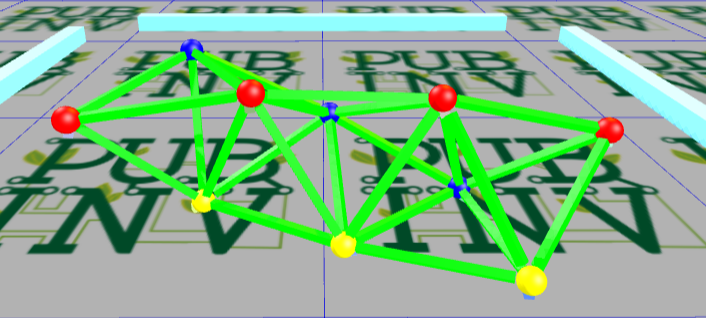
\includegraphics[width=0.4\textwidth]{figures/Tetrahelix0.png}
     \caption{Regular Tetrahelix}
\end{figure}

BC helix does not rest on a plane in a simple way. It is convenient to be able to ``untwist'' it and form a tetrahelix space frame that
has a flat planar surface. By making length changes in a certain way, we can untwist a tetrahelix to form a \emph{tetrabeam} which
has planar faces and has, for example, an equilateral triangular profile.

\section{A User's Formulation of the BC Helix}

If you can choose member lengths, you can form a linear combination of the equitetrabream lengths and the completely regular
lengths of the tetrahelix, thereby choosing the torsion.  If you are designing a space frame, this is a static design choice,
in a robot, it is a dynamic choice that can be used to twist the robot and/or exert torsion on the environment.

Ideally we would have a simple formula for defining the nodes based on any torsion we choose.
Unfortunately, it is not obvious that a linear combination of lengths produces a simple formula.
It is a goal of this paper to relate these two approaches to generating a tetrahelix continuum.

Coxeter constructs the BC helix\cite{coxeter1985simplicial} as a repeated rotation and translation of the tetrahedra, showing the
rotation is:
\[
\theta = \arccos(-2/3) 
\]
and the translation:
\[
h_{bc} = 1/\sqrt{10}
\]


$\theta$ is approximately $131.8103149$ degrees.
The angle $\theta$ is the rotation of a \emph{each} tetrahedra.
That is, a yellow tetrahedron is rotated slightly more than a $1/3$ of a revolution to match the face of the red tetrahedra.
$3 \theta - 2\pi$ is the apparent rotation of $V_3$ relative to $V_0$.

From Robert Gray's site, repeating formula by H.S.M. Coxeter:
\[
V(n) =
\left [
  \begin{tabular}{c}
   $ r_{bc} \cos(n \theta) $\\
   $ r_{bc} \sin(n \theta) $\\
   $ n h_{bc}  $
  \end{tabular}
  \right ],
\text{where:}
  \begin{tabular}{c}
 $ r_{bc} = \frac{3\sqrt{3}}{10} $\\
 $ h_{bc} = 1/\sqrt{10} $ \\
 $ \theta = \arccos(-2/3) $ \\
  \end{tabular}      
\]
where $n$ represents each integer numbered node in succession.

This formula defines a helix, but it is not any of the helices of the BC helix, but rather one that winds three times
as rapidly through all nodes. To a designer of tetrahelices, it is more natural to think of the three helices which
are visually apparent, that is, those three which are closely approximated by the by the outer edges or rails of the BC helix.

It is convenient to have a formula that gives us the nodes of just
each colored helix.
\[
H_{BCcolored}(n,c) = V(3n +c)
\]
where $c \in \{0,1,2\}$ specifies which of the rails is being computed.

Such a helix can be written:
\[
H_{BCcolored}(n,c) =
\left [
  \begin{tabular}{c}
   $ r_{bc}  \cos((3 \theta - 2 \pi)n + c  \theta $\\
   $ r_{bc} \sin((3 \theta - 2 \pi)n + c  \theta $\\
   $ (n + c/3) 3  h_{bc} $
  \end{tabular}
  \right ],
\text{where:}
  \begin{tabular}{c}
 $ r_{bc} = \frac{3\sqrt{3}}{10} $\\
 $ h_{bc} = 1/\sqrt{10} $ \\
 $ \theta = \arccos(-2/3) $ \\
  \end{tabular}      
  \]

In this formula, integral values of $n$ may be taken as a node number for one rail and used to compute its Cartesian
coordinates. Allowing $n$ to take non-integer values defines a continuous
helix in space which is close to the segmented polyline of the outer tetrahedra edges, and coincides with them at integer
values.
The parameter $c \in \{0,1,2\}$ specifies which of the rails is being computed.

The quantity $ (3 \theta - 2 \pi) \approx 35.43 \degree $, and is the angular shift between $V(n,color)$ and
$V(n+1,color)$. This quantity appears so often below that we call it the ``rail angle rho''. For the BC helix, $\rho_{bc} = (3 \theta - 2 \pi)$.

\begin{figure}[H]
  \label{railanglefig}
     \centering
     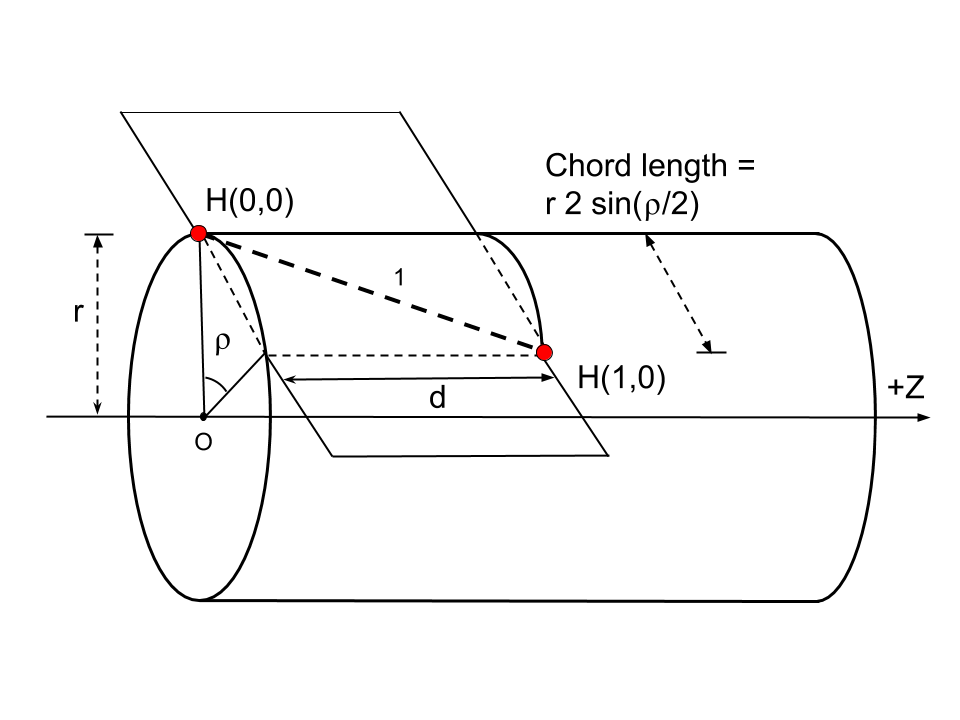
\includegraphics[width=0.7\textwidth]{figures/RailAngleGeometry.png}
     \caption{Rail Angle Geometry}
 \end{figure}

Since:
\[ \frac{2 \pi}{\rho_{bc}} \approx 10.16
\]
We can see that there are approximately $10.16$ red, blue or yellow tetrahedra on one rail in a single revolution.
The pitch of the Boerdijk--Coxeter helix of edge length $1$ is the length of three tetrahedra times this number:
\begin{align*}
  &= \frac{3 \cdot h_{bc} 2 \pi }{\rho_{bc}} \\
  &= \frac{3  \sqrt{\frac{2}{5}}  \pi}{\rho_{bc}} \\
  &\approx 9.6392 \\
\end{align*}
The pitch is less than the number of tetrahedra because the tetrahedra are not lined up perfectly.
It is a famous and interesting result that the pitch is irrational, a BC helix never has two tetrahedra
at precisely the same orientation around the $z$-axis. However, this is inconvenient to designers, who
might prefer a rational pitch. For example, a slight irregularity that led to a pitch of precisely 10 tetrahedra
in one revolution would allow an architect to design a column having a basis and a capital in the same relation to the tetrahedra
they touch.

A BC helix has the useful property that every member is precisely the same length. If we relax this, so that the tetrahedra it
comprises are not perfectly regular, then we can twist and curve the tetrahelix into a variety of shapes. This is useful to
the mechanical engineer or robotocist because the structure remains an inherently rigid, omni-triangulated space frame, which
may be expected to be at least somewhat mechanically strong.

\section{Optimal Tetrahelices Have Evenly Spaced Vertices}

We use the term \emph{tetrahelix} to mean any structure made of vertices and edges which is isomorphic to the BC helix,
in which the vertices lie on three helices, 
no matter what lengths the edges take on. One could consider various definitions of optimality for a tetrahelix,
but the must useful to an enginner is to minimize the maximum difference between any two edges. We call a
tetrahelix \emph{member-length minimax optimal} if there is not tetrahelix of the same radius and pitch with a smaller
maximum edge length difference.

Consider a tetrahelix isomporphic to an BC helix of unbounded extent. If all three rails do not have same pitch, there
is an edge of unbounded length. So we are justified in talking about the pitch of the tetrahelix, even though we think
of it as three helices. Similarly, if the axes are not parallel, there is an edge of unbounded length in the structure,
so it is not optimal.

Consider any tetrahelix in which the axes of the helices are parallel to $z$ but not coincident, but in which all three helices have the same
radius. Consider the projection along the $z$ axis, which will be a figure of dots and connecting segments in the $xy$ plane. The convex
hull for any one helix projection will be a circle (if its pitch is irrational) or an polygon if rational. So long as its rail angle is
not $0$, it will have at least two points in the plane. One of these will be longer and will be made shorter by moving that helix closer
to the midpoint of the other two in the $xy$ plane. Even if the rail angle is $\pi$, there will be two vertices for each rail, each of
which is connected to both vertices of the other two rails. At lesast one of these lines is a longest line which will be made shorter by moving
that helix in the $xy$ plane closer to the midpoint of the other two.

So any any optimal tetrahelix with a rail-angle of greater than $0$, that is, with any curvature, will have conincident axes.

We call a tetrahelix with $0$ curvature a \emph{tetrabeam}, and consider it as an important special case and an endpoint of a continuum
of tetrahelices of decreasing curvature.


 Now now that we have coincident axes, the same pitch, we can go on to the hard proof about where they occur.

 \begin{figure}[H]
     \centering
     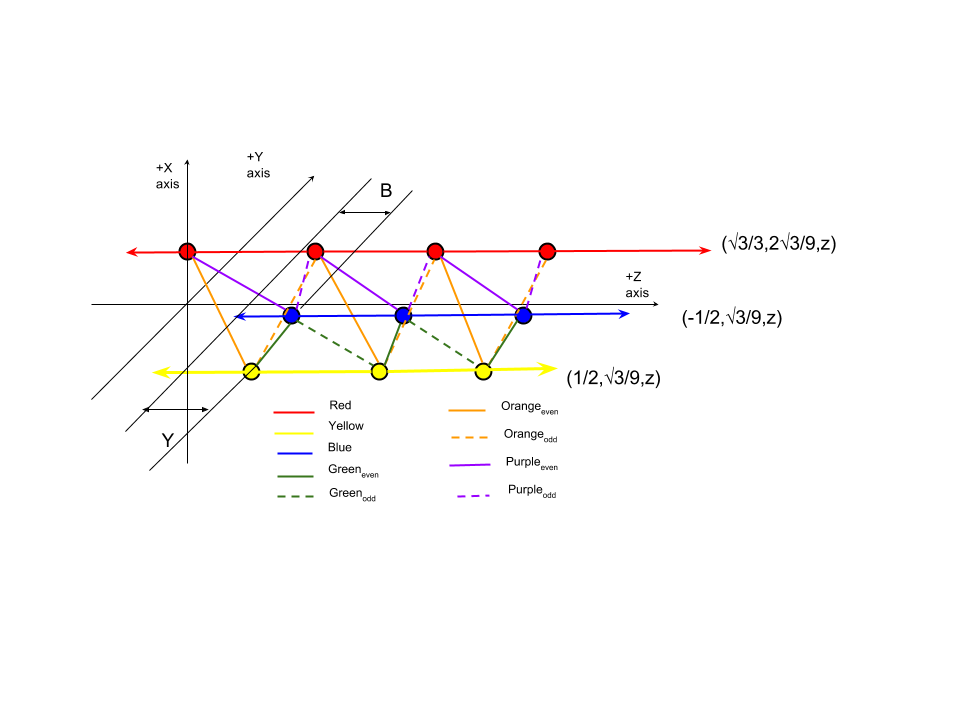
\includegraphics[width=0.9\textwidth]{figures/TetrahelixColoringDiagram.png}
     \caption{Coloring of an (untwisted) Tetrabeam}
 \end{figure}

 We show that in fact the nodes must be distributed in even thirds along the $z$-axis.

 Note that from the point of view of a single edge, we are on a slanted cylinder, when $\rho \neq 0$.
 This means for its point of view a cross section is an ellipse. So we have to be very careful in
 comparing lengths of edges relative to the tetrahedron, because a change in position along the edge
 changes the length of a line, but in a complicated way depending on where it is relative to the ellipse.

 \begin{theorem}
   \label{eventhirds}
   A tetrahelix of a given radius and height $h$ in which all nodes are evenly spaced at $h/3$ intervals on the $z$ axis is optimal.
     Any one tetrahedron in a tetrahelix has $1$ rail edge, $2$ one-hop edges connected to the rail and $2$ two-hop edges connected to the rail.
  The edge opposite of the rail edge is a one-hop edge.
  \end{theorem}

 \begin{proof}

   In principle in any tetrahelix where the three helices have any displacement along the $z$ axis there are 9 distinct edge classes:
   3 rail edges, a one-hop length between eachof 3 rails, and two hop length between each of three rails, where the two-hop length is a maximum
   length between rails (which could equal the one-hop length.) However, we have already shown the pitches and the rail lengths are equal
   in any optimal tetrahelix.
   
    Consider the tetrahelix in which the vertices  are evenly spaced at $h/3$ intervals on the $z$ axis. Every edge is either a rail edge, or it makes one
    hop, or it makes two hops. All of the one-hop edges are equal length.  All of the two-hop edges are equal length.
    
    Any displacemnt along the $z$ axis of any rail increases the length of one or two two-hop edges and shortens the length of one or two one-hop edges.
    This increases the minimax distance no matter what the rail edge length is, since all rail edges are the same length. Therefore, an evenly spaced
    tetrahelix is the unique optimal for any given radius and height.
  \end{proof}
  

Note that based on \ref{eventhirds}, we are justified in classifying edge lengths as \emph{rail},\emph{one-hop}, or
\emph{two-hops}. The one-hop edges are the edges between closest on the $z$-axis, and the two-hop edges are those that hop over a vertex.

By \ref{eventhirds} every optimal tetrahelix has vertices lying on helices expressible in the form:
\[
V_{optimal}(n,c) =
\left [
  \begin{tabular}{c}
   $ r \cos(n \alpha +  c 2 \pi /3)$\\
   $ r \sin(n \alpha +  c 2 \pi /3) $\\
   $ \frac{d(n +c / 3)}{3}   $
  \end{tabular}
  \right ],
\text{where:}
\begin{tabular}{c}
  $c \in \{0,1,2\}$
  \end{tabular}      
\]
where we have not yet investigated in the general case the relationships beteween $\alpha$, $r$, and $d$ in this formulation.
However, we understand that when $\alpha = 0$, the helices are degenerate, having curvature of $0$, and
we have the equitetrabeam.


This formulation $V(n,c)$ above is valuable, but obscures the essentially fact that the red, yellow, and blue helices distributed
about the central $z$ axis $120\degree$ from each other.
In order to rewrite this expression with an explicit rotation of $2\pi/3$, we expand 
the expression and seek to isolate the term $c2\pi/3$.
\begin{align*}
  \rho_{bc} n + c \theta  &=   \text{\{we aim for 3 in denominator, so we split...\}} \\
    (3 \theta - 2 \pi)n + (c/3)  (\theta /3)  &=   \text{\{we want $2\pi$ in numerator, so add canceling terms...\}} \\
  (3 \theta - 2 \pi)n + (c/ 3) (3 \theta - 2 \pi  + 2 \pi) &=  \text{\{associate...\}} \\
  (3 \theta - 2 \pi)n + (c/ 3) ((3 \theta - 2 \pi)  + 2 \pi) &=  \text{\{distribute...\}} \\  
  (3 \theta - 2 \pi)n + (c / 3) (3 \theta - 2 \pi)  + c 2 \pi /3 &=  \text{\{definition of $\rho_{bc}$...\}} \\
  \rho_{bc} n + (c / 3) \rho_{bc}  + c 2 \pi /3 &=  \text{\{collect like factors...\}} \\  
  \rho_{bc} (n + c/3)  + c 2 \pi /3  \\
\end{align*}
Now the the term on the left is the only one that depends on the scalar $n$. We use this to a create
a new formulation $H_{BCsymmetric}(n,c) = H_{colored}(n,c)$

The expression $n+c/3$ will now occur so often that we call it the ``c($\kappa$)olored number'' and we use the variable $\kappa$ to represent it: $\kappa = n+c/3$.
Recall that $c \in \{0,1,2\}$, but $n$ and $\kappa$ are are continuous (rational or real-valued.)

\[
H_{BCsymmmetric}(n,c) =
\left [
  \begin{tabular}{c}
   $ r  \cos(\rho_{bc} \kappa  + c 2 \pi /3) $\\
   $ r  \sin(\rho_{bc} \kappa  + c 2 \pi /3) $\\
   $ \kappa 3  h_{bc} $
  \end{tabular}
  \right ],
\text{where:}
  \begin{tabular}{c}
 $\kappa = n + c/3$ \\
    $\rho_{bc} = (3 \theta - 2 \pi)$ \\
    $ \theta = \arccos(-2/3) $
    $ h_{bc} = 1/\sqrt{10} $ \\    
  \end{tabular}      
\]

\section{Parametrizing Tetrahelices via Rail Angle}

Although the $\lambda$ parametrization presented above is a sensible one
because it unifies the BC-helix with the equitetrabeam, it is over-specific,
in that it makes a specific choice as to the relationship of the height $h$
to the radius $r$ which is somewhat arbitrary.

We seek a formula to generate optimal tetrahelices that accepts a
parameter that allows us to choose the tetrahelix conveniently. The
pitch of the helix is an obious choice, but is not defined when the
curvature is $0$, and important special case. The radius or the axial
distance between two nodes on the same rail are obvious choices, but
perhaps the clearest choice is to build formula that takes as its
input the ``rail angle'' $\rho$. We define $\rho$ to be the angle
formed in the X,Y plane $\angle R_i O R_{i+1}$ projecting out the $z$
axis and sighting along the positive $z$ axis. In other words, $\rho$
controls how far a rail edge of a tetrahelix deviates from being
parallel with the axis, or the ``twistiness'' of tetrahelix. Ideally
we will treat a positive angle as creating a clockwise tetrahelix and
a negative as creating a counter-clockwise helices.

Please refer back to Figure \ref{railanglefig}.

 These quantities are related by the expression:

\begin{align*}
  1^2 &= d^2 + (2 r \sin{ \rho / 2})^2 \\
  1 &= d^2 + 4 r^2 (\sin{ \rho / 2})^2 \\
  d^2 &= 1 - 4 r^2 (\sin{ \rho / 2})^2   
\end{align*}

Checking the important special case of the BC helix, we find that this equation
indeed holds true (treating $d$ in this equation as $3 h_{bc}$ as defined by
Gray and Coxeter, that is, $d_{bc} = 3h_{bc}$, where they are using it for the axial height from one node to
the next of a different color, but we use it to mean distance for the same color.

The rail angle $\rho$ also has the meaning that $2 \pi / \rho$ is the number of
tetraheda in a full revolution of the helix.

In choosing $\rho$, one greatly constrains $r$ and $h$, but does not completely
determine both of them together, so we treat both as parameters.

Rewriting our formulation in terms of $\rho$:
\[
H_{general}(n,c,\rho,d_{\rho},r_{\rho}) =
\left [
  \begin{tabular}{c}
   $ r_{\rho} \cos(\rho \kappa + c 2 \pi /3) $\\
   $ r_{\rho}  \sin(\rho \kappa + c 2 \pi /3) $\\
   $ d_{\rho} \kappa $
  \end{tabular}
  \right ],
\text{where:}
\begin{tabular}{c}
  $   1 = d_{\rho}^2 + 4 r_{\rho}^2 (\sin{ \rho / 2})^2 $ \\
    $\kappa = n + c/3$ \\
  \end{tabular}      
\]

$H_{general}$ generalizes $H_{continuum}$, but forces the user to select an $d_{\rho}$
which has a sensible radius, so it may be less convenient.

Note that when $\rho = 0$ then $h_{\rho} = 1$, but $r_{\rho}$ is not determined.

\begin{theorem}
  \label{generalformulaoptimal}
  The tetrahelices generated by $H_{general}$ are optimal in terms of minimum maximum member length when $r_{\rho}$ is chosen so that
  the length of the one-hop edge is equal to the rail length.
\end{theorem}

\begin{proof}
  This requires a minimax argument.
\end{proof}

By Theoerm \ref{eventhirds}, we can compute the (at most) three edge-lengths of an optimal
tetrahelix by (where $dist$ is the cartesian distance function):
\begin{align*}
  \text{rail} &= dist(H_{general}(n,c,\rho,d_{\rho},r_{\rho}),H_{general}(n+1,c,\rho,d_{\rho}),r_{\rho})) = 1 \\
  \text{one-hop} &= dist(H_{general}(n,c,\rho,d_{\rho},r_{\rho}),H_{general}(n,c+1,\rho,d_{\rho},r_{\rho}))  \\
  \text{two-hops} &= dist(H_{general}(n,c,\rho,d_{\rho},r_{\rho}),H_{general}(n,c+2,\rho,d_{\rho},r_{\rho}))  \\  
\end{align*}
Which are invarinat for all $n$ and $c$.

\begin{align*}
  \text{one-hop} &= dist(H_{general}(n,c,\rho,d_{\rho}),H_{general}(n,c+1,\rho,d_{\rho}),r_{\rho})  \\
  \text{one-hop} &= dist(H_{general}(0,0,\rho,d_{\rho}),H_{general}(0,1,\rho,d_{\rho},r_{\rho}))  \\  
  \text{one-hop}  &= \sqrt{\frac{d_{\rho}^2}{9} + (r_{\rho}\sin(\rho((1/3)\cdot 0 + 0)) - r_{\rho}\sin(\rho((1/3)\cdot 0 + 1)+\frac{2\pi}{3}))^2  +
    (r_{\rho}\cos(\rho((1/3)\cdot0+0)) - r_{\rho}\cos(\rho((1/3)\cdot 0+1) + \frac{2\pi}{3})))^2} \\
  \text{one-hop}  &= \sqrt{\frac{d_{\rho}^2}{9} + (0  - r_{\rho}\sin(\rho/3 + \frac{2\pi}{3}))^2  +
    (r_{\rho} - r_{\rho}\cos(\rho/3 + \frac{2\pi}{3}))^2} \\
  \text{one-hop}  &= \sqrt{\frac{d_{\rho}^2}{9} + r_{\rho}^2\sin^2(\rho/3 + \frac{2\pi}{3})  +
    r_{\rho}^2(1 - \cos(\rho/3 + \frac{2\pi}{3}))^2} \\
  \text{one-hop}  &= \sqrt{\frac{d_{\rho}^2}{9} + r_{\rho}^2(\sin^2(\rho/3 + \frac{2\pi}{3})  + (1 - \cos(\rho/3 + \frac{2\pi}{3}))^2)} \\
  \text{but... } & d_{\rho}^2 &= 1 - 4 r_{\rho}^2 (\sin{ \rho / 2})^2 \\
  \text{one-hop}  &= \sqrt{\frac{1 - 4 r_{\rho}^2 (\sin{ \rho / 2})^2}{9} + r_{\rho}^2(\sin^2(\rho + \frac{2\pi}{3})  + (1 - \cos(\rho + \frac{2\pi}{3}))^2)} \\  
\end{align*}

To Be Done: I need to see if the one-hop formulat can be simplified.
Compute the two-hop formula and test that it gives length 1 when the BC constants. -- YES!

By similar algebra and trigonometry:
\begin{align*}
  \text{two-hops}  &= \sqrt{4\frac{1 - 4 r_{\rho}^2 (\sin{ \rho / 2})^2}{9} + r_{\rho}^2(\sin^2(2\rho/3 + \frac{4\pi}{3})  + (1 - \cos(2\rho/3 + \frac{4\pi}{3}))^2)} \\
\end{align*}

Note: it is not clear I am allowed to do this, because the two-hop function is different!

Let $f_{\rho} = \sin^2(\rho/3 + \frac{2\pi}{3})  + (1 - \cos(\rho/3 + \frac{2\pi}{3})^2$.
Let $g_{\rho} = \sin^2(2\rho/3 + \frac{4\pi}{3})  + (1 - \cos(2\rho/3 + \frac{4\pi}{3})^2$.

The expression $f_{\rho}$ is maximized when $\rho = 2\pi/6 = 60\degree$, so that
is in some sense the ``wildest'' rail angle which maximizes the lengths. Since this expression is increasing up until this angle,
we conclude that:
\begin{align*}
  \text{two-hops} - \text{one-hop}  &= \sqrt{\frac{4d_{\rho}^2}{9} + r_{\rho}^2g_{\rho}} - \sqrt{\frac{d_{\rho}^2}{9} + r_{\rho}^2f_{\rho}} 
\end{align*}

To Be Done: I need to plot this expression, see if it has a maximum, and see if it always decreasing in this range, to see if we can prove optimality.

Since $d_{\rho}$ and $r_{\rho}$ are positive, this difference decreases as $f_{\rho}$ increases. Therefore we decrease the minimax length
of the whole system as we increase $\rho$ up to $\pi/3$ up unto the point that the shorter, one-hop distance is equal to the rail-length ($1$).
Therefore, to optimize the whole system so long as $\rho < \pi/3$, we equate one-hop to $1$ to find the optimum radius:


\begin{align*}
  1 &= \sqrt{\frac{d_{\rho}^2}{9} + r_{\rho}^2(\sin^2(\rho/3 + \frac{2\pi}{3})  + (1 - \cos(\rho/3 + \frac{2\pi}{3}))^2)} \\
  r_{\rho} &= \frac{2 \sqrt{2} }{\sqrt{9 \sqrt{3} sin(\rho/3) + 9 \cos(\rho/3) + 2 cos(\rho)+ 16 }}
\end{align*}
(where $9 \cos(\rho/3) + 2 cos(\rho)+ 16  \neq 0$), which does not occur when $\rho \leq \pi/3$).

Therefore, by computing $r_{\rho}$ from this equation, we can construct minimax optimal tetrahelix for an $\rho < \pi/3$.

(Note: This fails the check of computing the BC radius for the BC rail angle.)



\section{The Equitetrabeam}

Just as $H_{general}$ constructs the BC helix (with careful and non-obvious choices of parameters) which is an important
special case due to its regularity, it constructs an additional special (degenerate) case when the rail angle $\rho = 0$
and $d = 1$ (the edgelength), where the cross sectional area is an equilateral triangle of unchanging orientation.
We call this the \emph{equitetrabeam}.

However, choosing $d = 1$ and $\rho = 0$ does not fix the radius. We would like to choose the radius so that the
minimax difference between the lengths is as small as possible.


 \begin{figure}[H]
     \centering
     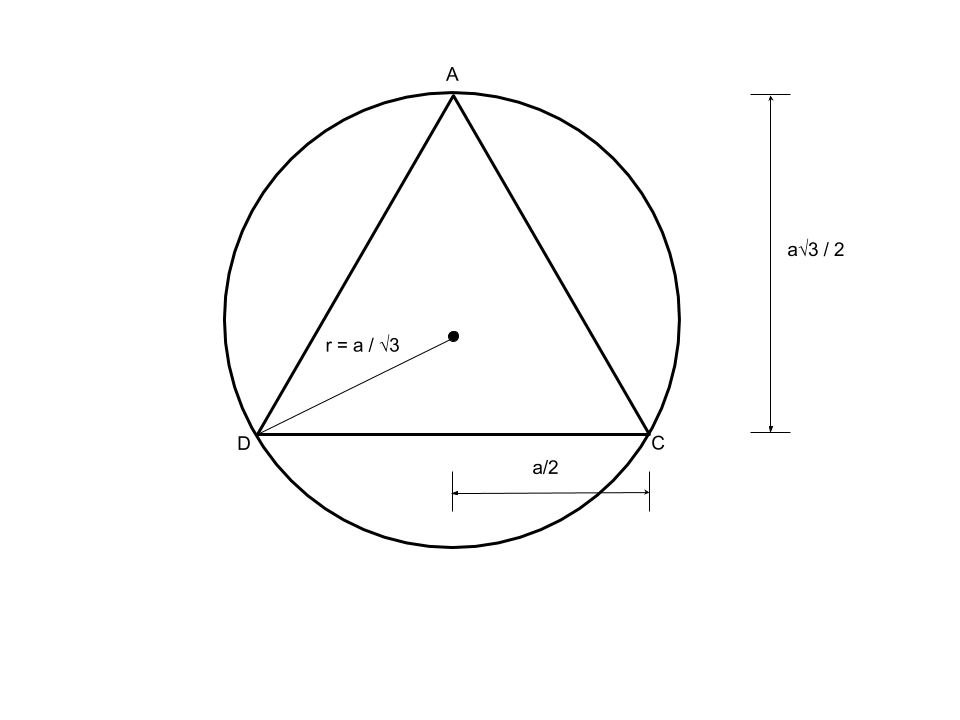
\includegraphics[width=0.9\textwidth]{figures/EquilateralDiagram.png}
     \caption{Coloring of an (untwisted) Tetrabeam}
 \end{figure}


\begin{theorem}
The equitetrabeam with minimal maximal edge difference is produced by $H_{general}$ when $ r = \sqrt{\frac{8}{27}} $.
  \end{theorem}

When $\rho = 0$, our formulae for distances are particular simple. Let $a$ be the length of the equilateral triangle
forming the beam cross section. Then by geometry $r = a \sqrt{3}$.
\begin{align*}
  \text{rail} &=  1 \\
  \text{one-hop} &= \sqrt{\frac{1}{9} + 3r^2}\\
\text{two-hops}    &= \sqrt{\frac{4}{9} + 3r^2}
\end{align*}
Computing the derivative of two-hops - one-hop:
\begin{align*}
 \frac{\partial \text{two-hops} - \text{one-hop}}{r} &= \frac{\partial \sqrt{4/9 + 3r^2} - \sqrt{1/9 + 3r^2}}{\partial r} \\
  \frac{\partial \text{two-hops} - \text{one-hop}}{r} &= 9r (\frac{1}{\sqrt{27r^2 + 4}} - \frac{1}{\sqrt{ 27r^2 + 1}}) 
\end{align*}
which is negative for all $r> 0$. Thererfore two-hop - one-hop
is minimized when we maximize $r$, up until one-hop = rail.

Note that two-hops increases more and more slowly as $r$ increases. Therefore the minimum maximum will
be obtained with the value of $r$ that when $one-hop = 1$. This can be observed from the
plot of two-hops - one-hops as a function of $r$, or by observing that the derivate of two-hops - one-hop
is negative for $r > 0$. (That is, the value of one-hop increases faster than two-hops.) 
Setting the one-hop distance to $d = 1$ also has the pleasing property of giving us only two lengths. Then
\begin{align*}
   1  &=  \sqrt{\frac{1}{9} + 3r^2} \\
   r  &= \sqrt{\frac{8}{27}} \\
   r &\approx 0.5443
\end{align*}

This radius produces a two-hop rail length of
$\frac{2}{\sqrt{3}}$. The difference between this 
and $1$ of $\approx 15.47\% $.

Note: Another interesting solution is derived by setting (one-hop + two-hop)/2 = 1,  occurs at $r = \sqrt{35}/4$,
which produces three length classes of $11/12, 12/12, 13/12$.



\section{Adding an Untwisting Parameter}

We observe that it by thinking of the straight lines of the Equitetrabeam as a degenerate helix of zero curvature,
it should be possible to define a smoothly varying continuum between the Boerdijk--Coxeter helix and the Equitetrabeam and every
curvature and torsion between the two.

We seek to unify this with degenerate helix formula for the equitetrabeam:
\[
H_{etb}(n,c) =
\left [
  \begin{tabular}{c}
   $ r_{etb}  \cos( 0 \cdot \kappa  + c 2 \pi /3) $\\
   $ r_{etb}  \sin( 0 \cdot \kappa  + c 2 \pi /3) $\\
   $ \kappa d_{etb} $
  \end{tabular}
\right ],
\text{where:}
  \begin{tabular}{c}
 $\kappa = n + c/3$ \\
    $\rho_{bc} = (3 \theta - 2 \pi)$ \\
   $ \theta = \arccos(-2/3) $
  \end{tabular}      
\]
where $ r_{etb} = \sqrt{\frac{8}{27}}$, $d_{etb} = 1$,

Now basic components of the helix, which are the radius $r$, the rate of rotation, and the rate of
axial growth can all be linearly interpolated with a parameter $\lambda$ between their high values (for the BC helix)
and low values (for the equitetrabeam):

\begin{align*}
r_{\lambda}  &=  \lvert \lambda \rvert \cdot (\frac{3 \sqrt{3}}{10}  - \sqrt{\frac{8}{27}}) + \sqrt{\frac{8}{27}}  \\
d_{\lambda} &=   \lvert \lambda \rvert \cdot (3 \sqrt{10} - 1) + 1 \\
\phi_{\lambda} &=  \lambda \cdot \rho_{bc}  + 0
\end{align*}
to create a formula that generates a continuum of tetrahedral structures:

\[
H_{continuum}(n,c,\lambda) =
\left [
  \begin{tabular}{c}
   $ r_{\lambda} \cos(\phi_{\lambda} \kappa + c 2 \pi /3) $\\
   $ r_{\lambda}  \sin(\phi_{\lambda} \kappa + c 2 \pi /3) $\\
   $ d_{\lambda} \kappa $
  \end{tabular}
  \right ],
\text{where:}
  \begin{tabular}{c}
    $\kappa = n + c/3$ \\
    $ \phi_{\lambda} =  \lambda \rho_{bc}  + 0 $\\
    $\rho_{bc} = (3 \theta - 2 \pi)$ \\
   $ \theta = \arccos(-2/3) $
  \end{tabular}      
\]
A value of $\lambda = 0$ generates the equitetrabeam, and $\lambda = 1$ generates the Boerdijk--Coxeter helix, and every
value $\lambda \in [-1,1]$ generates an attractive structure which if physically realized is an inherently rigid structure
with member lengths of no greater disparity than $16\%$.
In the sense of structural engineering, it would be a relatively strong space frame. When $\lvert \lambda \rvert > 1$, tetrahelices
are still produced, but as $\lvert \lambda \rvert >> 2$ these tetrahelices probably cease to be interesting to mechanical engineers,
because their ability to withstand axial forces seem to diminish significantly.

 \begin{figure}[H]
     \centering
     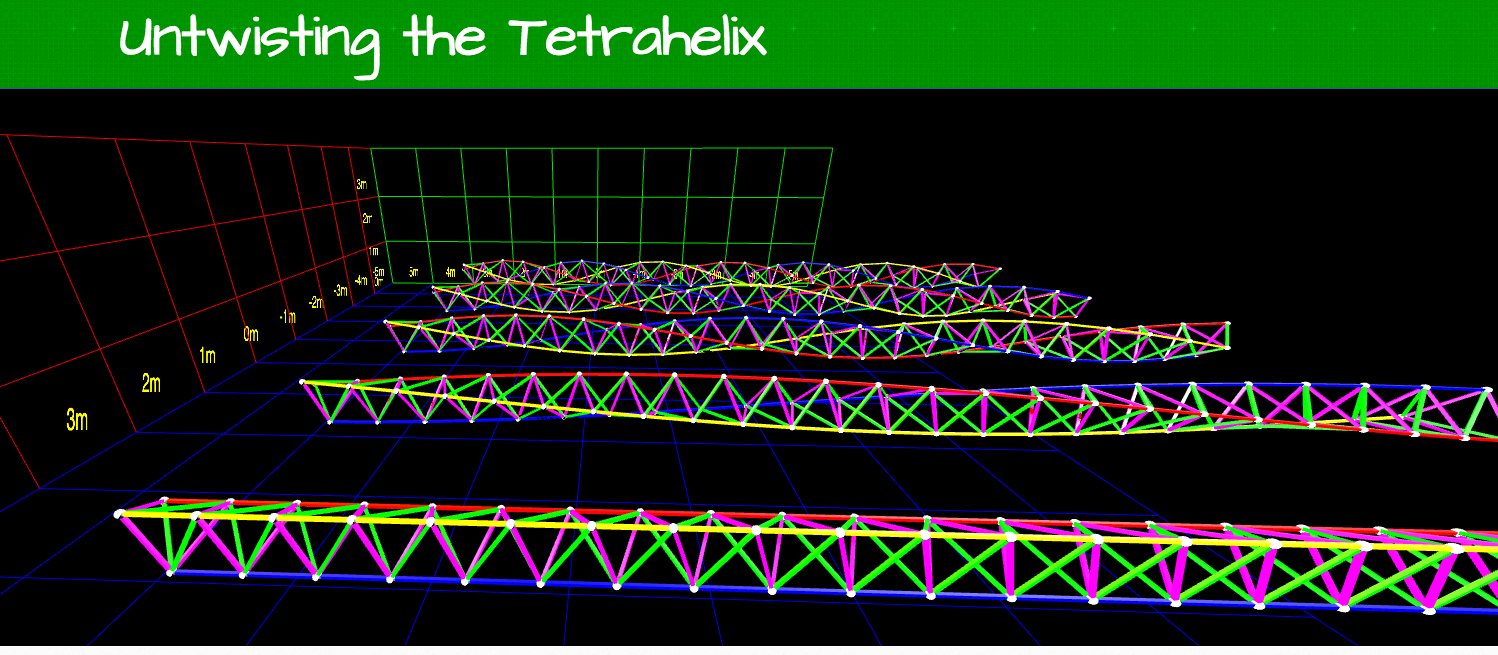
\includegraphics[width=0.9\textwidth]{figures/Continuum.png}
     \caption{A Continuum of Tetrahelices}
 \end{figure}


Negative values of $\lambda$ generate clockwise tetrahelices; positive generate counter-clockwise helices.

Furthermore, this formula allows one to design the pitch (in edge length units) as a function of $\lambda$ of the helix (along one rail)
where $\lambda \neq 0$:
\[
p(\lambda) = 2 \pi  \cdot \frac{(\frac{8}{27} -1) \lambda +1)}{ \lambda  \rho_{bc} }
\]

We can then create a continuum of radius, length, rho to place into our general equation
to create continuum of helices between the BC and equitetrabeam. This continuum is 
minimax-length optimal at its endpoints, and may be optimal throughout. This untwisting is accomplished
only by changing the length of the two-hop member.

\section{Utility for Robotics}

Trusses and space frames remain an important design field in mechanical and structural engineering\cite{mikulas1985sequentially},
including deployable and moving trusses\cite{claypool2012readily}.

Starting twenty years ago, Sanderson\cite{sanderson1996modular}, Hamlin,\cite{TetrobotBook}, and others including Lee\cite{lee2002dynamic}
created a style of robotics based on changing the lengths of members
joined at the center of a joint, thereby creating a connection to pure geometry. More recently NASA has experimented with
tensegrities\cite{NTRT}, a different point in the same design spectrum. These fields create a need to explore the notion of
geometries changing over time, not generally considered directly by pure geometry.

As suggested by Buckminster Fuller, the most convenient geometries to consider are those that have regular member
lengths, in order to facilitate the inexpensive manufacture and construction of the robot.  In a plane, the octet truss
is such a geometry, but in a line, the Boerdijk--Coxeter helix is a regular structure.

However, a robot must move, and so it is interesting to consider the transmutations of these geometries, which was in
fact the motivation for creating the equitetrabream.

\begin{theorem}
  By changing only the length of the members that change rails and make two nodes, you can untwist a tetrobot
  form the Boerdijk-Coxeter configuration to the equitetrabeam which rests flat on the plane.
\end{theorem}

\begin{proof}
  Proof by our computer program that does this by forming a linear interpolation of links.
\end{proof}

\begin{figure}[H] %float with two figures
  \centering
     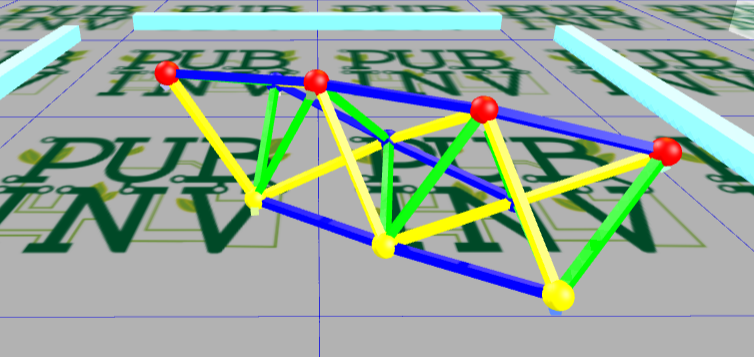
\includegraphics[width=0.4\textwidth]{figures/Tetrahelix1.png}
     \caption{2/3rd Twisted Tetrahelix}
     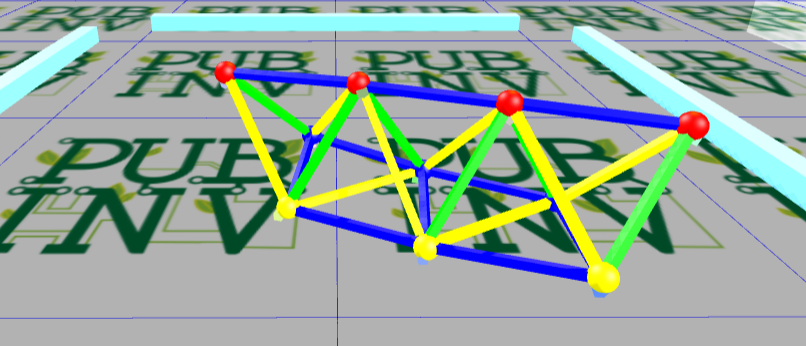
\includegraphics[width=0.4\textwidth]{figures/Tetrahelix2.png}
     \caption{1/3rd Twisted, 2/3rd Untwisted Tetrahelix}
     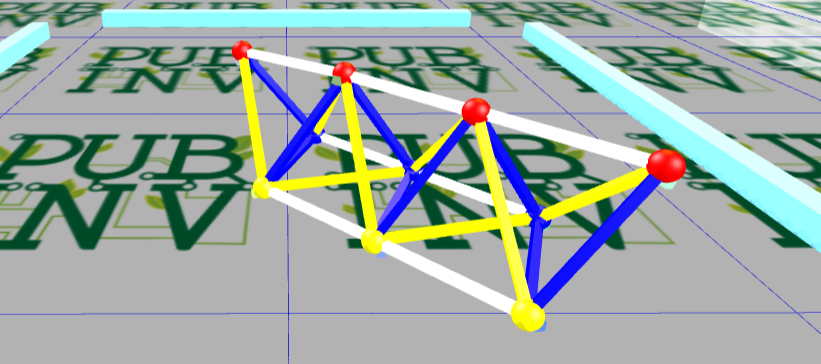
\includegraphics[width=0.4\textwidth]{figures/Tetrahelix3.png}
     \caption{The Equitetrabream: Fully Untwisted Tetrahelix}
\end{figure}

\section{Contact and Getting Involved}

The Gluss Project \url{http://pubinv.github.io/gluss/}
is a free-libre, open-source research, hardware, and software project that welcomes volunteers.
It is our goal to organize projects for the benefit of all humanity without seeking profit or intellectual property.
To assist, contact \href{mailto:read.robert@gmail.com}{$<$read.robert@gmail.com$>$}.

\bibliographystyle{IEEEtran}
\bibliography{IEEEabrv,gluss}

\end{document}

TODO:

See if we can accurately compute the derivative of two-hop - one-hop and if it is always negative, meaning that
it is always optimal to set one-hop = 1.  The we have a way to compute one-hope.

Remove the weirdly colored diagram.

Add to the rail angle diagram.

Note that Lamba = 16 almost produces a 2-rail helicoid.

When abs(lambda) > 4, we seem to have marked differences in the parameters. Understand why this is and what is causing it.
(it is possible that positive and negative rho values behave very differently?

Note: Would be really nice to have the GUI show you all computed parameters.

Note: Distance is clearly lower on first computations..

Create working toolkit for desin/exploration.

Improve code that way, use white background, floor.

Figure out if I am computing something wrong.



Try to compute optimal radius within our context. This would let us assert that we have
an ``optimum'' continuum.  Not worth much to an engineer, but valuable.

Review and continue editing, being careful to introduce concepts in the correct order.

On Rail diagram, add a second tetrahedron, and a second rho.



Make YouTube video.


    \section{Old Proofs}
    
We can create the distance between representative nodes as:
\begin{align*}
  \overline{\rm AB}  &= 1 \\        
  \overline{\rm CD}  &= \sqrt{G^2 + r^2(1 + -\cos{2 G \rho})} \\
  \overline{\rm AC}  &= \sqrt{O^2 + r^2(1 + \sin^2{O \rho}  - \cos^2{O \rho})} \\  
  \overline{\rm AC}  &= \sqrt{O^2 + r^2(1 + -\cos{2 O  \rho})} \\
  \overline{\rm BD}  &= \sqrt{P^2 + r^2(1 + -\cos{2 P \rho}))} \\
  \overline{\rm AD}  &= \sqrt{(O+G)^2 + r^2(1 + -\cos{2 (O + G)  \rho})} \\
  \overline{\rm BC}  &= \sqrt{(P+G)^2 + r^2(1 + -\cos{2 (P + G) \rho})} \\      
\end{align*}


Using the cartesian distance formula:
\begin{align*}
  \overline{\rm CD}  &= \sqrt{G^2 + (r\sin{0 \rho} -  r\sin{G \rho})^2 + (r\cos{0 \rho} - r\cos{G \rho})^2} \\
    \overline{\rm CD}  &= \sqrt{G^2 + (0 -  r\sin{G \rho})^2 + (r - r\cos{G \rho})^2} \\
    \overline{\rm CD}  &= \sqrt{G^2 + r^2(\sin{G \rho})^2 + r^2(1 - \cos{G \rho})^2} \\
    \overline{\rm CD}  &= \sqrt{G^2 + r^2(1 + \sin^2{G \rho}  - \cos^2{G \rho})} \\
    \overline{\rm CD}  &= \sqrt{G^2 + r^2(1 + -\cos{2 G \rho})} \\        
\end{align*}
Note: $\sin^2{x \rho}  - \cos^2{x \rho} = -\cos{2 x \rho}$

So, for all O,G,P,
\begin{align*}
  \overline{\rm AB}  &= 1 \\        
  \overline{\rm CD}  &= \sqrt{G^2 + r^2(1 + -\cos{2 G \rho})} \\
  \overline{\rm AC}  &= \sqrt{O^2 + r^2(1 + \sin^2{O \rho}  - \cos^2{O \rho})} \\  
  \overline{\rm AC}  &= \sqrt{O^2 + r^2(1 + -\cos{2 O  \rho})} \\
  \overline{\rm BD}  &= \sqrt{P^2 + r^2(1 + -\cos{2 P \rho}))} \\
  \overline{\rm AD}  &= \sqrt{(O+G)^2 + r^2(1 + -\cos{2 (O + G)  \rho})} \\
  \overline{\rm BC}  &= \sqrt{(P+G)^2 + r^2(1 + -\cos{2 (P + G) \rho})} \\      
\end{align*}




Then we can simplify our distance equations:
\begin{align*}
  \overline{\rm AB}  &= 1 \\        
  \overline{\rm CD}  &= \sqrt{G^2 + r^2(1 + -\cos{2 G \rho})} \\
  \overline{\rm AC} &=   \overline{\rm BD} &= \sqrt{P^2 + r^2(1 + -\cos{2 P \rho}))} \\
  \overline{\rm AC} &=   \overline{\rm BD} &= \sqrt{((1-G)/2)^2 + r^2(1 + -\cos{ \rho (1-G) }))} \\  
  \overline{\rm AD} &=  \overline{\rm BC} &=  \sqrt{((P+G)^2 + r^2(1 + -\cos{2 (P + G) \rho})} \\
  \overline{\rm AD} &=  \overline{\rm BC} &=  \sqrt{((1+ G)/2 )^2 + r^2(1 + -\cos{\rho (1 + G)})} \\        
\end{align*}

When $G = 0$, $\overline{\rm CD} = 0$. Our solution is improved as we increase $G$ until either $ \overline{\rm CD} = \overline{\rm AC}$, or the
quantity $ \overline{\rm BC} - \overline{\rm CD} $ starts increasing rather than decreasing (that is, when the derivative is positive.)



Suppose $\overline{\rm C'D'}$ is the shortest edge. Increasing $G$ thereby improves our mimimum, up until the next shortest edge length, $\overline{\rm AC}$.
This may increase $\overline{\rm BC}$ and $\overline{\rm AD}$, but more slowly (???) than $\overline{\rm C'D'}$ is being increased, until  $\overline{\rm C'D'} =
\overline{\rm AC}$.
Note: This is sketchy, can we show that the derivative of our formula for CD  with respect to $G$ is really higher than $AD$? These derivatives will depend on $\rho$ slightly, which is exactly right!

\begin{align*}
  \text{rail} &=  1 \\
  \text{one-hop} &= \sqrt{\frac{1}{3}^2 + (\frac{3a}{2\sqrt{3}})^2 + (a/2)^2}\\
\text{one-hop}  &= \sqrt{\frac{1}{9} + a^2} \\
    \text{two-hops} &= \sqrt{\frac{2}{3}^2 + (\frac{3a}{2\sqrt{3}})^2 + (a/2)^2}  \\
\text{two-hops}    &= \sqrt{\frac{4}{9} + a^2}
\end{align*}
Computing the derivative of two-hops - one-hop:
\begin{align*}
 \frac{\partial \text{two-hops} - \text{one-hop}}{a} &= \frac{\partial \sqrt{4/9 + a^2} - \sqrt{1/9 + a^2}}{\partial a} \\
  \frac{\partial \text{two-hops} - \text{one-hop}}{a} &= \frac{a}{\sqrt{a^2 + 4/9}} - \frac{a}{\sqrt{ a^2 + 1/9}} 
\end{align*}

  

  
